\documentclass[10pt, aspectratio=169]{beamer}

% Beamer theme and colors
\usetheme{Madrid} 
\useinnertheme{rounded}

% Custom engaging colors (Blue & Slate)
\definecolor{coolBlue}{RGB}{20, 80, 140} 
\definecolor{coolSlate}{RGB}{40, 50, 60}
\definecolor{lightGray}{RGB}{245, 245, 245}

\setbeamercolor{palette primary}{bg=coolBlue, fg=white}
\setbeamercolor{palette secondary}{bg=coolSlate, fg=white}
\setbeamercolor{palette tertiary}{bg=coolSlate!80!black, fg=white}
\setbeamercolor{structure}{fg=coolBlue}

\setbeamercolor{block title}{bg=coolSlate, fg=white}
\setbeamercolor{block body}{bg=lightGray, fg=black}

\setbeamercolor{title}{bg=coolBlue, fg=white}
\setbeamercolor{frametitle}{bg=coolBlue, fg=white}


\usepackage[utf8]{inputenc}
\usepackage{amsmath, amssymb}
\usepackage{amsthm}
\usepackage{tikz}
\usetikzlibrary{arrows.meta, angles, quotes, calc, positioning}

\title{Cops and Robbers: A Graph Theory Game}
\author[The American University in Cairo]{Bassel M. Shoeib \and Mahmoud H. AlAskndrani \\ \and Michael R. Guirgis \and Mohamed A. AboElFotouh}
\institute[]{The American University in Cairo}
\date{Spring 2026}

\begin{document}

\begin{frame}
    \titlepage
\end{frame}

\begin{frame}{Outline}
    \tableofcontents
\end{frame}

\section{Introduction}

\begin{frame}{Motivation}
    \begin{itemize}
        \item Imagine a city with a single cop actively pursuing a robber.
        \item Both know the city layout and each other's location.
        \item They take alternating turns moving to adjacent locations.
        \item \textbf{Question:} Can the robber escape safely and outrun the cop?
        \item We model this using a connected, simple, finite graph $G(V, E)$.
    \end{itemize}
\end{frame}

\begin{frame}{The Game of Cops and Robbers}
    \begin{alertblock}{The Game}
    Let $G(V, E)$ be a connected, simple, finite graph. The rules are:
    \begin{enumerate}
        \item \textbf{Starting Positions:} Cop chooses $c_0 \in V(G)$, then robber chooses $r_0 \in V(G)$.
        \item \textbf{Movement:} Players move alternately, cop goes first. A player at $x$ can move to adjacent $y$ (where $xy \in E(G)$) or stay at $x$.
        \item \textbf{Perfect Information:} Both players know the graph structure and each other's position at all times.
    \end{enumerate}
    \end{alertblock}
\end{frame}

\begin{frame}{Cop-win and Robber-win Graphs}
    \begin{block}{Cop-win Graph}
        A graph $G$ is \textit{cop-win} if there is a winning strategy for the cop, meaning the cop guarantees $c_t = r_t$ for some finite turn $t$.
    \end{block}

    \begin{exampleblock}{Robber-win Graph}
        A graph $G$ is \textit{robber-win} if there is a winning strategy for the robber, meaning the robber guarantees $c_t \neq r_t$ for all turns $t \ge 0$.
    \end{exampleblock}
\end{frame}

\section{Fundamental Results}

\begin{frame}{Basic Lemmas}
    \begin{lemma}
        All complete graphs $K_n$ are cop-win graphs.
    \end{lemma}
    \textit{Proof Idea:} Cop starts anywhere. Robber picks a vertex. Cop catches robber on the first move since all vertices are adjacent.
    
    \vspace{0.5cm}
    \begin{lemma}
        All trees are cop-win graphs.
    \end{lemma}
    \textit{Proof Idea:} There is a unique path between any two vertices in a tree. The cop simply takes the unique path towards the robber, strictly decreasing the distance at each step.
\end{frame}

\begin{frame}{Cycles are Robber-win}
    \begin{lemma}
        All cycles of length at least 4 are robber-win graphs.
    \end{lemma}
    \textit{Proof Idea:}
    \begin{itemize}
        \item Robber starts at distance $\ge 2$ from the cop (possible since $n \ge 4$).
        \item Every vertex has exactly two neighbors.
        \item The robber simply moves in the opposite direction of the cop.
        \item The cop can never decrease the distance to $0$, avoiding capture indefinitely.
    \end{itemize}
\end{frame}

\section{Characterization of Cop-win Graphs}

\begin{frame}{Pitfalls}
    To formalize a general characterization, we define a \textit{pitfall}.
    \begin{alertblock}{Pitfall}
        A vertex $u \in V$ is a \textbf{pitfall} (or corner) if there exists a distinct vertex $v \in N(u)$ such that its closed neighborhood is a subset of the closed neighborhood of $v$, i.e., $N[u] \subseteq N[v]$. We say $v$ \textbf{dominates} $u$.
    \end{alertblock}
    \begin{block}{Intuition}
        If the robber is at a pitfall $u$, and the cop is at the dominating vertex $v$, the cop can reach any vertex the robber could move to, guaranteeing capture.
    \end{block}
\end{frame}

\begin{frame}{The Dismantlability Theorem}
    \begin{theorem}
        A finite graph is cop-win \textbf{iff} it can be reduced to a single vertex through the successive removal of pitfalls.
    \end{theorem}
    \textit{Forward Direction ($\Rightarrow$):}
    \begin{itemize}
        \item Consider the turn before capture. Cop at $v$ must be able to reach any vertex robber at $u$ can move to.
        \item This implies $N[u] \subseteq N[v]$, meaning $u$ is a pitfall.
        \item Removing $u$ preserves the strategy, so the graph is dismantlable.
    \end{itemize}
\end{frame}

\begin{frame}{The Dismantlability Theorem (cont.)}
    \textit{Backward Direction ($\Leftarrow$):}
    \begin{itemize}
        \item Proceed by induction by removing pitfall $u$ dominated by $v$ to get restricted graph $G'$.
        \item Construct a mapping $f(x)$ mapping $u$ to $v$.
        \item The cop chases the "shadow" robber on the smaller cop-win graph $G'$.
        \item Once caught in $G'$, if the real robber is at $u$, they are immediately caught from $v$ as $N[u] \subseteq N[v]$.
    \end{itemize}
\end{frame}

\section{Multiple Cops}

\begin{frame}{The Cop Number}
    \begin{alertblock}{Cop Number}
        The cop number of a graph $G$, denoted $\mathcal{C}(G)$, is the minimum number of cops required to guarantee catching the robber.
    \end{alertblock}
    \begin{itemize}
        \item Note that $\mathcal{C}(G) \le \beta(G)$, where $\beta(G)$ is the domination number of $G$.
        \item If the cops form a dominating set, they can capture the robber in one step.
    \end{itemize}
\end{frame}

\begin{frame}{Isometric Path Lemma}
    \begin{lemma}[Isometric Path Lemma]
        Let $P$ be a shortest path between vertices $u, v \in V(G)$. With at least two cops in play, one cop on $P$ can prevent the robber from ever entering $P$. (If the robber steps on $P$, they are immediately caught).
    \end{lemma}
    \textit{Proof Sketch:}
    \begin{itemize}
        \item Cop maintains strategy ensuring $d(c,z) \le d(r,z)$ for all $z \in V(P)$.
        \item If the robber threatens $z_0 \in V(P)$ by decreasing distance, the cop moves towards $z_0$.
        \item Robber cannot threaten two vertices $x, y$ on opposite sides of the cop simultaneously, as $P$ is a shortest path (violates triangle inequality).
        \item Thus, if the robber steps on $z \in V(P)$, $d(c,z) \le d(r,z) = 0$, meaning the cop captures them.
    \end{itemize}
\end{frame}

\begin{frame}{Planar Graphs}
    \begin{theorem}[Aigner and Fromme]
        Any planar graph $G$ has $\mathcal{C}(G) \le 3$.
    \end{theorem}
    \begin{itemize}
        \item \textit{Idea:} Use 2 cops to control two shortest paths meeting at a vertex, forming a territorial boundary.
        \item Use the Jordan Curve Theorem on these paths and the 3rd cop on a crossing path to strictly reduce the robber's bounded territory at each stage.
        \item Eventually, the territory is strictly reduced until the robber is caught.
    \end{itemize}
\end{frame}

\begin{frame}{Jordan Curve Illustration}
    \begin{center}
    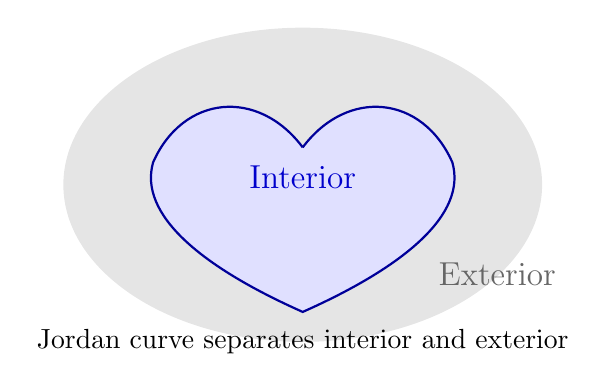
\begin{tikzpicture}[scale=0.95]
        % exterior oval (gray) surrounding the interior
        \fill[gray!20] (0,0.1) ellipse (3.2cm and 2.1cm);

        % heart-like interior shape (filled)
        \fill[blue!12] (0,0.6) .. controls (0.6,1.4) and (1.6,1.3) .. (2.0,0.4)
            .. controls (2.2,-0.3) and (1.35,-1.0) .. (0,-1.6)
            .. controls (-1.35,-1.0) and (-2.2,-0.3) .. (-2.0,0.4)
            .. controls (-1.6,1.3) and (-0.6,1.4) .. (0,0.6) -- cycle;

        \draw[blue!60!black, thick]
            (0,0.6) .. controls (0.6,1.4) and (1.6,1.3) .. (2.0,0.4)
            .. controls (2.2,-0.3) and (1.35,-1.0) .. (0,-1.6)
            .. controls (-1.35,-1.0) and (-2.2,-0.3) .. (-2.0,0.4)
            .. controls (-1.6,1.3) and (-0.6,1.4) .. (0,0.6);

        % Labels
        \node[blue!80!black] at (0,0.2) {\large Interior};
        \node[gray!80!black] at (2.6,-1.1) {\large Exterior};
        \node at (0,-2.0) {Jordan curve separates interior and exterior};
    \end{tikzpicture}
    \end{center}
\end{frame}

\begin{frame}{Robber Territory: Reachable Zone}
    \begin{center}
    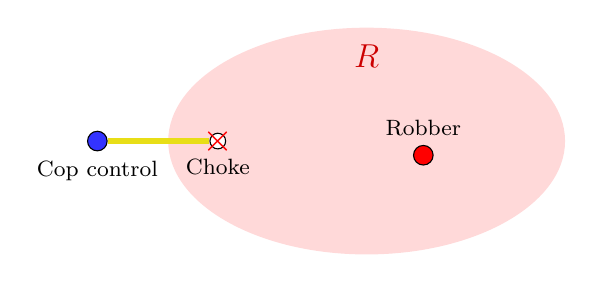
\begin{tikzpicture}[scale=0.9]
        % Territory blob
        \fill[red!15] (0, 0) ellipse (2.8cm and 1.6cm);
        \node[red!80!black, font=\large] at (0, 1.2) {$R$};

        % Nodes
        \node[circle, fill=white, draw=black, inner sep=2pt, label=below:{\footnotesize Choke}] (choke) at (-2.1, 0) {};
        \node[circle, fill=blue!80, draw=black, inner sep=2.5pt, label=below:{\footnotesize Cop control}] (blocker) at (-3.8, 0) {};
        \node[circle, fill=red, draw=black, inner sep=2.5pt, label=above:{\footnotesize Robber}] (robber) at (0.8, -0.2) {};

        % Blocked path/gate
        \draw[yellow!90!black, line width=2pt] (blocker) -- (choke);
        \node[red, font=\Large] at (-2.1, 0) {$\times$}; % Blocked indicator
    \end{tikzpicture}
    \end{center}
\end{frame}

\begin{frame}{Case A: One Bottleneck Toward the Territory}
    \begin{center}
    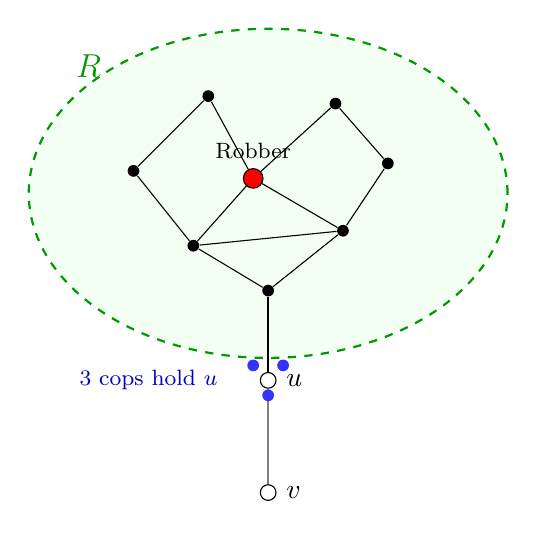
\begin{tikzpicture}[scale=0.95]
        % Territory boundary (dashed to indicate a region)
        \fill[green!5] (0, 1.5) ellipse (3.2cm and 2.2cm);
        \draw[green!60!black, thick, dashed] (0, 1.5) ellipse (3.2cm and 2.2cm);
        \node[green!60!black, font=\large] at (-2.4, 3.2) {$R$};

        % Net-like nodes inside the territory
        \node[circle, fill=black, inner sep=1.5pt] (n1) at (0, 0.2) {};
        \node[circle, fill=black, inner sep=1.5pt] (n2) at (-1, 0.8) {};
        \node[circle, fill=black, inner sep=1.5pt] (n3) at (1, 1.0) {};
        \node[circle, fill=black, inner sep=1.5pt] (n4) at (-1.8, 1.8) {};
        \node[circle, fill=black, inner sep=1.5pt] (n5) at (-0.2, 1.7) {};
        \node[circle, fill=black, inner sep=1.5pt] (n6) at (1.6, 1.9) {};
        \node[circle, fill=black, inner sep=1.5pt] (n7) at (-0.8, 2.8) {};
        \node[circle, fill=black, inner sep=1.5pt] (n8) at (0.9, 2.7) {};
        
        % Edges inside territory to make it "net-like"
        \draw (n1) -- (n2); \draw (n1) -- (n3);
        \draw (n2) -- (n4); \draw (n2) -- (n5);
        \draw (n3) -- (n5); \draw (n3) -- (n6);
        \draw (n4) -- (n7); \draw (n5) -- (n7); 
        \draw (n5) -- (n8); \draw (n6) -- (n8);
        \draw (n2) -- (n3); % Extra cross-connection

        % Robber node placed on one of the inner nodes
        \node[circle, fill=red, draw=black, inner sep=2.5pt, label=above:{\footnotesize Robber}] (robber) at (n5) {};

        % Bottleneck node u
        \node[circle, fill=white, draw=black, inner sep=2pt, label=right:$u$] (u) at (0, -1.0) {};
        
        % Connection from bottleneck into the territory
        \draw[thick] (u) -- (n1);

        % Rest of the graph (v) going downwards
        \node[circle, fill=white, draw=black, inner sep=2pt, label=right:$v$] (v) at (0, -2.5) {};
        \draw[gray, thick] (u) -- (v);

        % 3 Cops stationed at the bottleneck u
        \node[circle, fill=blue!80, inner sep=1.5pt] at (-0.2, -0.8) {};
        \node[circle, fill=blue!80, inner sep=1.5pt] at (0.2, -0.8) {};
        \node[circle, fill=blue!80, inner sep=1.5pt] at (0, -1.2) {};
        \node[blue!80!black, font=\footnotesize] at (-1.6, -1.0) {3 cops hold $u$};
        
    \end{tikzpicture}
    \end{center}
\end{frame}

\begin{frame}{Case B(i): Cycle with Disjoint External Component}
    \begin{center}
    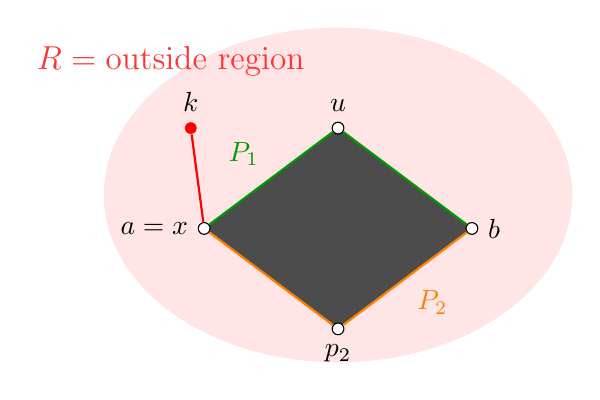
\begin{tikzpicture}[scale=0.85]
        % Background territory blob
        \fill[red!10] (0, 0.5) ellipse (3.5cm and 2.5cm);
        \node[red!80, font=\large] at (-2.5, 2.5) {$R = \text{outside region}$};
      
        % Cycle interior
        \fill[black!70] (-2, 0) -- (0, 1.5) -- (2, 0) -- (0, -1.5) -- cycle;
      
        % Nodes
        \node[circle, fill=white, draw=black, inner sep=1.5pt, label=above:$u$] (u) at (0, 1.5) {};
        \node[circle, fill=white, draw=black, inner sep=1.5pt, label=left:{$a=x$}] (a) at (-2, 0) {};
        \node[circle, fill=white, draw=black, inner sep=1.5pt, label=right:$b$] (b) at (2, 0) {};
        \node[circle, fill=white, draw=black, inner sep=1.5pt, label=below:$p_2$] (p2) at (0, -1.5) {};
        \node[circle, fill=red, inner sep=1.5pt, label=above:$k$] (k) at (-2.2, 1.5) {};
      
        % Paths
        \draw[green!60!black, thick] (a) -- (u) node[midway, above left=1pt] {$P_1$} -- (b);
        \draw[orange, thick] (a) -- (p2) -- (b) node[midway, below right=1pt] {$P_2$};
        \draw[red, thick] (a) -- (k);
    \end{tikzpicture}
    \end{center}
\end{frame}

\begin{frame}{Case B(ii): Path Q Splitting the Cycle}
    \begin{center}
    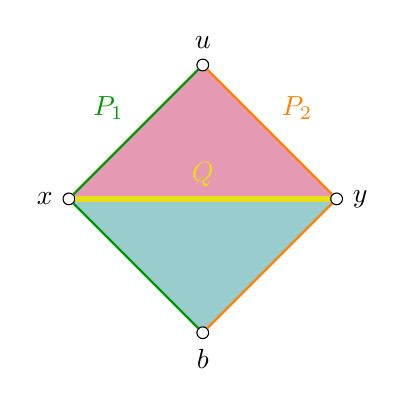
\begin{tikzpicture}[scale=0.85]
        % Region fills
        \fill[purple!40] (-2, 0) -- (0, 2) -- (2, 0) -- cycle;
        \fill[teal!40] (-2, 0) -- (0, -2) -- (2, 0) -- cycle;
      
        % Nodes
        \node[circle, fill=white, draw=black, inner sep=1.5pt, label=above:$u$] (u) at (0, 2) {};
        \node[circle, fill=white, draw=black, inner sep=1.5pt, label=below:$b$] (b) at (0, -2) {};
        \node[circle, fill=white, draw=black, inner sep=1.5pt, label=left:$x$] (x) at (-2, 0) {};
        \node[circle, fill=white, draw=black, inner sep=1.5pt, label=right:$y$] (y) at (2, 0) {};
      
        % Paths
        \draw[green!60!black, thick] (u) -- (x) node[midway, above left=1pt] {$P_1$} -- (b);
        \draw[orange, thick] (u) -- (y) node[midway, above right=1pt] {$P_2$} -- (b);
        \draw[yellow!90!black, line width=2pt] (x) -- (y) node[midway, above] {$Q$};
    \end{tikzpicture}
    \end{center}
\end{frame}

\begin{frame}{Case B(ii) Details: Path Q Starting from A}
    \begin{center}
    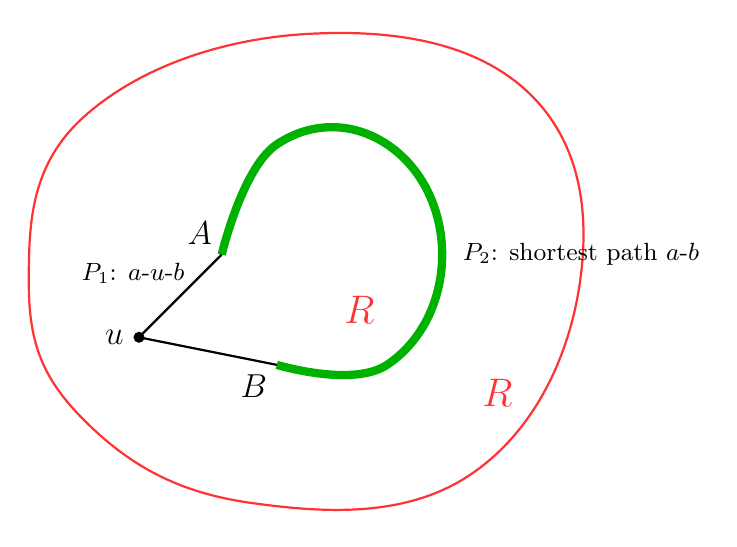
\begin{tikzpicture}[x=0.7cm,y=0.7cm]
        % 1. Outer Red Region
        \draw[red!80, thick] plot [smooth cycle, tension=0.7] coordinates {
            (-5,0) (-4,3) (0,4.5) (4,3.5) (5,0) (3,-3.5) (-1,-4) (-4,-2.5)
        };

        % 2. Coordinate Definitions
        \coordinate (A) at (-1.5, 0.5);
        \coordinate (B) at (-0.5, -1.5);
        \coordinate (U) at (-3, -1);
        \coordinate (RightEdge) at (2.5, 0.5);

        % 3. Inner Green Region (OPEN curve, gap between A and B)
        \draw[green!70!black, line width=3pt] plot [smooth, tension=0.75] coordinates {
            (A) (-0.5,2.5) (1.5,2.5) (RightEdge) (1.5,-1.5) (B)
        };
        
        % 4. Node 'u'
        \fill (U) circle (2pt) node[left, xshift=-2pt, font=\large] {$u$};

        % 5. Path P1
        \draw[thick] (U) -- (A);
        \draw[thick] (U) -- (B);
        \node[above left, font=\small] at (-2, -0.2) {$P_1$: $a$-$u$-$b$};

        % 6. Path Q (Straight edge starting at A)
        %\draw[thick] (A) -- (RightEdge) coordinate[pos=0.5] (MidQ);
        
        % 7. Label Q 
        %\node[above, font=\large] at (MidQ) {$Q$};
        \node[right, font=\small] at (2.7, 0.5) {$P_2$: shortest path $a$-$b$};

        % 8. Labels A and B
        \node[above left, font=\large] at (A) {$A$};
        \node[below left, font=\large] at (B) {$B$};

        % 9. Red 'R' Regions
        \node[red!80, font=\Large] at (1, -0.5) {$R$};
        \node[red!80, font=\Large] at (3.5, -2) {$R$};
    \end{tikzpicture}
    \end{center}
\end{frame}

\begin{frame}{Case B(ii) Details: Path Q Starting from u}
    \begin{center}
    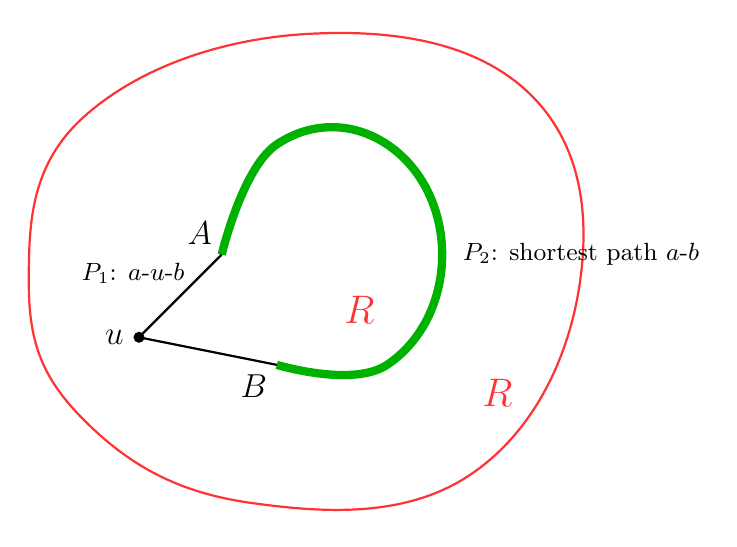
\begin{tikzpicture}[x=0.7cm,y=0.7cm]
        % 1. Outer Red Region
        \draw[red!80, thick] plot [smooth cycle, tension=0.7] coordinates {
            (-5,0) (-4,3) (0,4.5) (4,3.5) (5,0) (3,-3.5) (-1,-4) (-4,-2.5)
        };

        % 2. Coordinate Definitions
        \coordinate (A) at (-1.5, 0.5);
        \coordinate (B) at (-0.5, -1.5);
        \coordinate (U) at (-3, -1);
        \coordinate (RightEdge) at (2.5, 0.5);

        % 3. Inner Green Region (OPEN curve, gap between A and B)
        \draw[green!70!black, line width=3pt] plot [smooth, tension=0.75] coordinates {
            (A) (-0.5,2.5) (1.5,2.5) (RightEdge) (1.5,-1.5) (B)
        };
        
        % 4. Node 'u'
        \fill (U) circle (2pt) node[left, xshift=-2pt, font=\large] {$u$};

        % 5. Path P1
        \draw[thick] (U) -- (A);
        \draw[thick] (U) -- (B);
        \node[above left, font=\small] at (-2, -0.2) {$P_1$: $a$-$u$-$b$};

        % 6. Path Q (Straight edge starting at u, crossing between A and B)
        %\draw[thick] (U) -- (RightEdge) coordinate[pos=0.6] (MidQ);
        
        % 7. Label Q 
        %\node[above, font=\large, yshift=2pt] at (MidQ) {$Q$};
        \node[right, font=\small] at (2.7, 0.5) {$P_2$: shortest path $a$-$b$};

        % 8. Labels A and B
        \node[above left, font=\large] at (A) {$A$};
        \node[below left, font=\large] at (B) {$B$};

        % 9. Red 'R' Regions
        \node[red!80, font=\Large] at (1, -0.5) {$R$};
        \node[red!80, font=\Large] at (3.5, -2) {$R$};
    \end{tikzpicture}
    \end{center}
\end{frame}

\begin{frame}{A Lower Bound Theorem}
    \begin{theorem}
        Any graph $G$ with no 3-cycles or 4-cycles and $\delta(G) \ge n$ has $\mathcal{C}(G) \ge n$.
    \end{theorem}
    \begin{itemize}
        \item \textit{Proof Sketch:} Place $n-1$ cops.
        \item The robber can find a vertex $r$ not dominated by any of the $n-1$ cops.
        \item Due to the absence of 3- and 4-cycles, after cops move, at most $n-1$ of the robber's neighbors are threatened.
        \item Since the robber has at least $n$ neighbors (min degree $\ge n$), there is always at least one safe neighbor to continually move to!
    \end{itemize}
\end{frame}

\begin{frame}{Tightness of Planar Bound}
    \begin{center}
        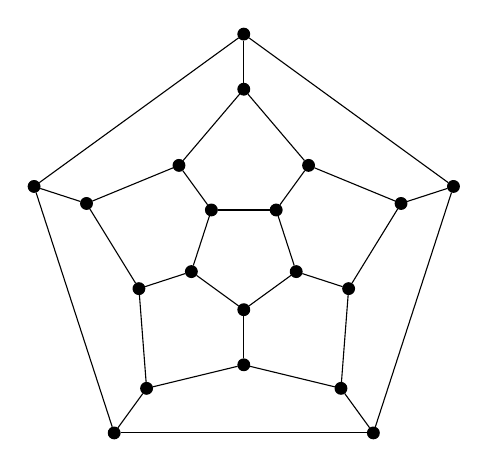
\begin{tikzpicture}[scale=0.7, every node/.style={circle, draw, fill=black, inner sep=1.5pt}]
            \foreach \i in {1,...,5} {
                \node (a\i) at (162 - \i*72: 4) {};
                \node (b\i) at (162 - \i*72: 3) {};
                \node (c\i) at (126 - \i*72: 2) {};
                \node (d\i) at (126 - \i*72: 1) {};
            }
            
            \foreach \i in {1,...,5} {
                \pgfmathsetmacro{\next}{int(mod(\i,5)+1)}
                \pgfmathsetmacro{\prev}{int(mod(\i+3,5)+1)}
                \draw (a\i) -- (a\next);
                \draw (d\i) -- (d\next);
                \draw (a\i) -- (b\i);
                \draw (c\i) -- (d\i);
                \draw (b\i) -- (c\i);
                \draw (b\i) -- (c\prev);
            }
        \end{tikzpicture}
    \end{center}
    This planar graph has no 3- or 4-cycles, and $\delta(G)=3$. By our previous theorem, $\mathcal{C}(G) \ge 3$, proving the planar bound is tight.
\end{frame}

\section{Conclusion}

\begin{frame}{Conclusion}
    \begin{itemize}
        \item The game of Cops and Robbers intimately connects pursuit-evasion dynamics with structural graph theory.
        \item \textbf{Single Cop:} Cop-win graphs are exactly those that are dismantlable via pitfalls.
        \item \textbf{Multiple Cops:} The minimum degree in graphs with large girth limits the cop number from below.
        \item \textbf{Planarity:} Topologically, planar graphs drastically restrict evasion, capping the cop number at 3.
    \end{itemize}
    \vspace{1cm}
    \begin{center}
        \Large \textbf{Thank You!}
    \end{center}
\end{frame}

\end{document}